{\fontsize{12pt}{22pt} \textbf{Distribution functions}\par}

\vspace{5mm}

Mass function

The probability mass function (p.m.f.) is the histogram of the distribution, that is:

- x-axis: values

- y-axis: frequency

\vspace{5mm}

Density function

The probability density function (p.d.f.) is the "smooth histogram" of the distribution.

\vspace{5mm}

\begin{center}
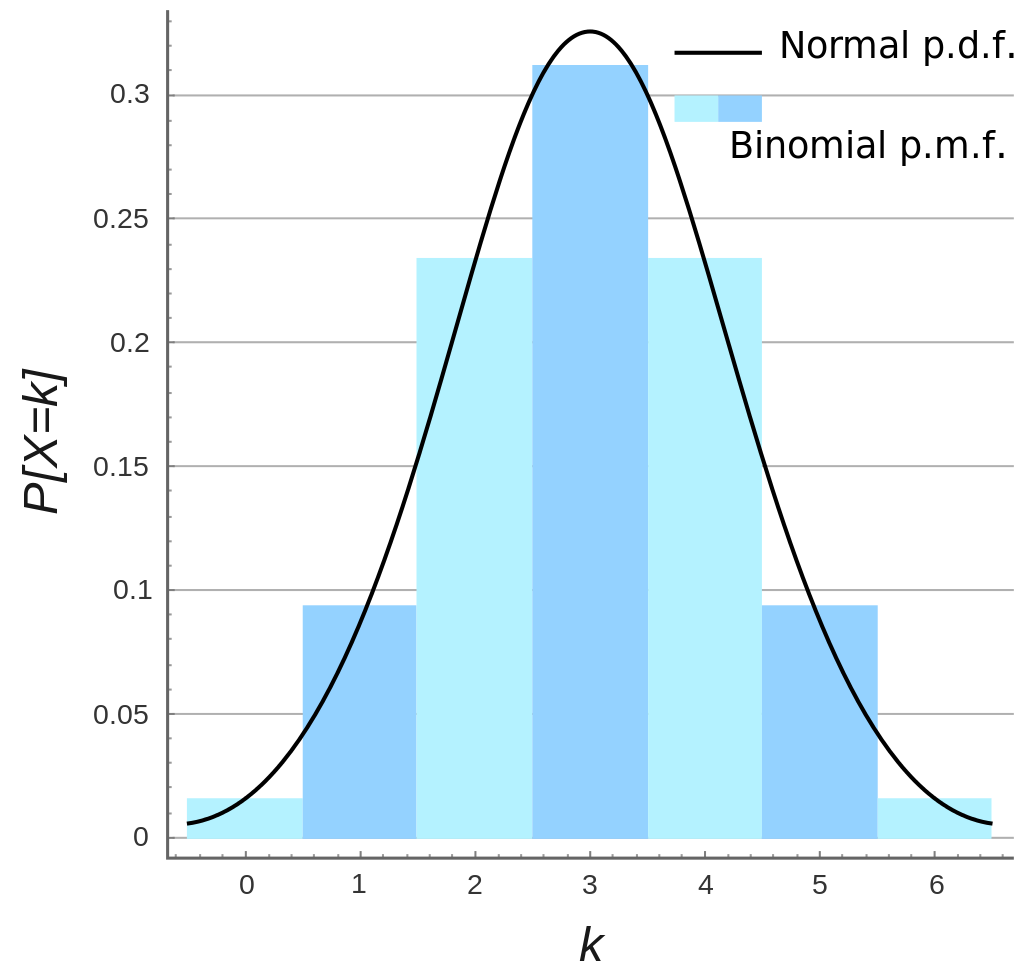
\includegraphics[scale=0.15]{mass_density_functions.png}
\end{center}

\vspace{5mm}

Cumulative distribution function

The cumulative distribution function (c.d.f) is given by $F_X(x)= \mathbb{P}(X < x)$. 

The empirical distribution function is its estimation:
$\widehat{F}_n(x) = \frac{1}{n}\{\text{number of elements} < x\}$

\begin{center}
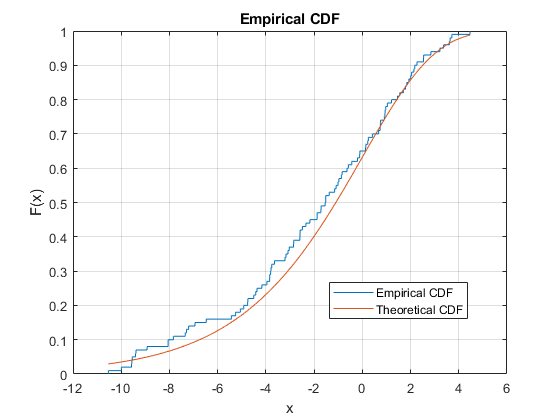
\includegraphics[scale=0.4]{CDF.png}
\end{center}

\vspace{5mm}